% Created 2021-02-11 Thu 15:13
% Intended LaTeX compiler: pdflatex
\documentclass[11pt]{article}
\usepackage[hyphens]{url}
\usepackage{float}
\usepackage[utf8]{inputenc}
\usepackage[T1]{fontenc}
\usepackage{graphicx}
\usepackage{grffile}
\usepackage{longtable}
\usepackage{wrapfig}
\usepackage{rotating}
\usepackage[normalem]{ulem}
\usepackage{amsmath}
\usepackage{textcomp}
\usepackage{amssymb}
\usepackage{capt-of}
\usepackage{hyperref}
\author{Tigany Zarrouk\thanks{tigany.zarrouk@kcl.ac.uk}}
\date{15.04.2020}
\title{Tight-binding investigation of defects in Ti.}
\hypersetup{
 pdfauthor={Tigany Zarrouk},
 pdftitle={Tight-binding investigation of defects in Ti.},
 pdfkeywords={},
 pdfsubject={},
 pdfcreator={Emacs 27.1 (Org mode 9.4.4)}, 
 pdflang={English}}
\begin{document}

\maketitle


\section*{Motivation}
\label{sec:org028837a}
\begin{itemize}
\item Titanium alloys are used in highly demanding circumstances.
\item Brittle oxide layer can crack.
\item Solutes affect dislocation mobility, causing hardening.
\item Interaction between oxygen and dislocation cores is not clear.
\item Need for atomistic modelling.
\item Exploration of Ti/oxide scale interface will give insights into oxygen
diffusion, oxygen induces brittleness and stress corrosion cracking in Ti
alloys.
\end{itemize}
\begin{NOTES}
\begin{itemize}
\item Corrosion resistance, high strength to weight ratio.
\item Ti is used in commercial jet airliners
\end{itemize}
\end{NOTES}


\section*{Quantum Methods}
\label{sec:org4ebdaa8}
\begin{itemize}
\item Density Functional Theory is not feasible.
\item System size is limited due to computational cost.
\item Boundaries of cell affect relaxation of core more.
\item Semi-empirical method is more computationally efficient.
\end{itemize}

\subsection*{Tight Binding}
\label{sec:org36f8108}


\begin{itemize}
\item Tight binding is an approximation to DFT.
\item Overlaps between atomic orbitals are key parameters.
\item Parameters can be fitted to experimental data
\item \(\mathcal{O}(N^3)\), but much smaller prefactor compared to DFT.
\end{itemize}

\subsection*{BOP}
\label{sec:orgd919a42}

\begin{itemize}
\item BOP is a faster but less accurate \(\mathcal{O}(N)\) method of interatomic
force calculation within tight-binding.
\item One builds a local density of states from moments, giving detailed
electronic structure information.
\end{itemize}


\subsection*{Embedding}
\label{sec:org76df04e}

\begin{itemize}
\item Idea is to combine speed of BOP (\(\mathcal{O}(N)\)) with accuracy of
tight-binding \(\mathcal{O}(N^3)\).
\item Increasing the number of atoms gives freedom to:
\begin{itemize}
\item Investigate isolated dislocations.
\item Include solutes at more realistic concentrations.
\item Simulate interfaces near a surface (e.g. TiO\(_2\) and
bulk Ti)
\end{itemize}
\end{itemize}
\begin{NOTES}
Invariance theorem with green's function approaches. So good with boundary
conditions. 
\end{NOTES}


\section*{Parameter Optimisation}
\label{sec:org3d958e7}
\begin{itemize}
\item Parameter set for TB model optimised by two evolutionary algorithms:
particle swarm and covariance matrix evolution.
\item Fitting targets were a mix of experimental and DFT data.
\end{itemize}

\subsection*{Results of optimisation.}
\label{sec:orgbed67c2}
\begin{center}
\begin{tabular}{lrr}
\hline
Quantity & TB & target (DFT + empirical)\\
\hline
\(a_{\alpha}\)              [bohr] & 5.585 & 5.577\\
\((c/a)_{\alpha}\) & 1.583 & 1.587\\
\(C_{11}\)                  [GPa ] & 171.6 & 176.1\\
\(C_{33}\)                  [GPa ] & 198.9 & 190.5\\
\(C_{44}\)                  [GPa ] & 47.4 & 50.8\\
\(C_{12}\)                  [GPa ] & 94.7 & 86.9\\
\(C_{13}\)                  [GPa ] & 61.2 & 68.3\\
\(a_{\omega}\)              [bohr] & 8.93 & 8.73\\
\(c_{\omega}\)              [bohr] & 5.39 & 5.32\\
\(a_{\beta}\)               [bohr] & 6.20 & 6.18\\
bandwidth                 [Ryd ] & 4.65 & 4.97\\
\hline
\end{tabular}
\end{center}

\subsubsection*{Energy Splittings}
\label{sec:orgf21683c}

\begin{center}
\begin{tabular}{lrr}
\hline
Quantity & TB & target\\
\hline
\(\Delta E(\omega-\alpha)\)     [mRyd ] & 0.53 & -0.73\\
\(\Delta E(\text{4H}-\alpha)\)  [mRyd ] & 1.58 & 3.17\\
\(\Delta E(\text{6H}-\alpha)\)  [mRyd ] & 2.48 & 3.72\\
\(\Delta E(\text{fcc}-\alpha)\) [mRyd ] & 3.78 & 4.52\\
\(\Delta E(\beta-\alpha)\)      [mRyd ] & 5.35 & 7.64\\
\hline
\end{tabular}
\end{center}



\section*{Phonon Spectra}
\label{sec:org308d6d3}

\subsection*{\(\alpha\) phase}
\label{sec:org92876f7}
\begin{center}
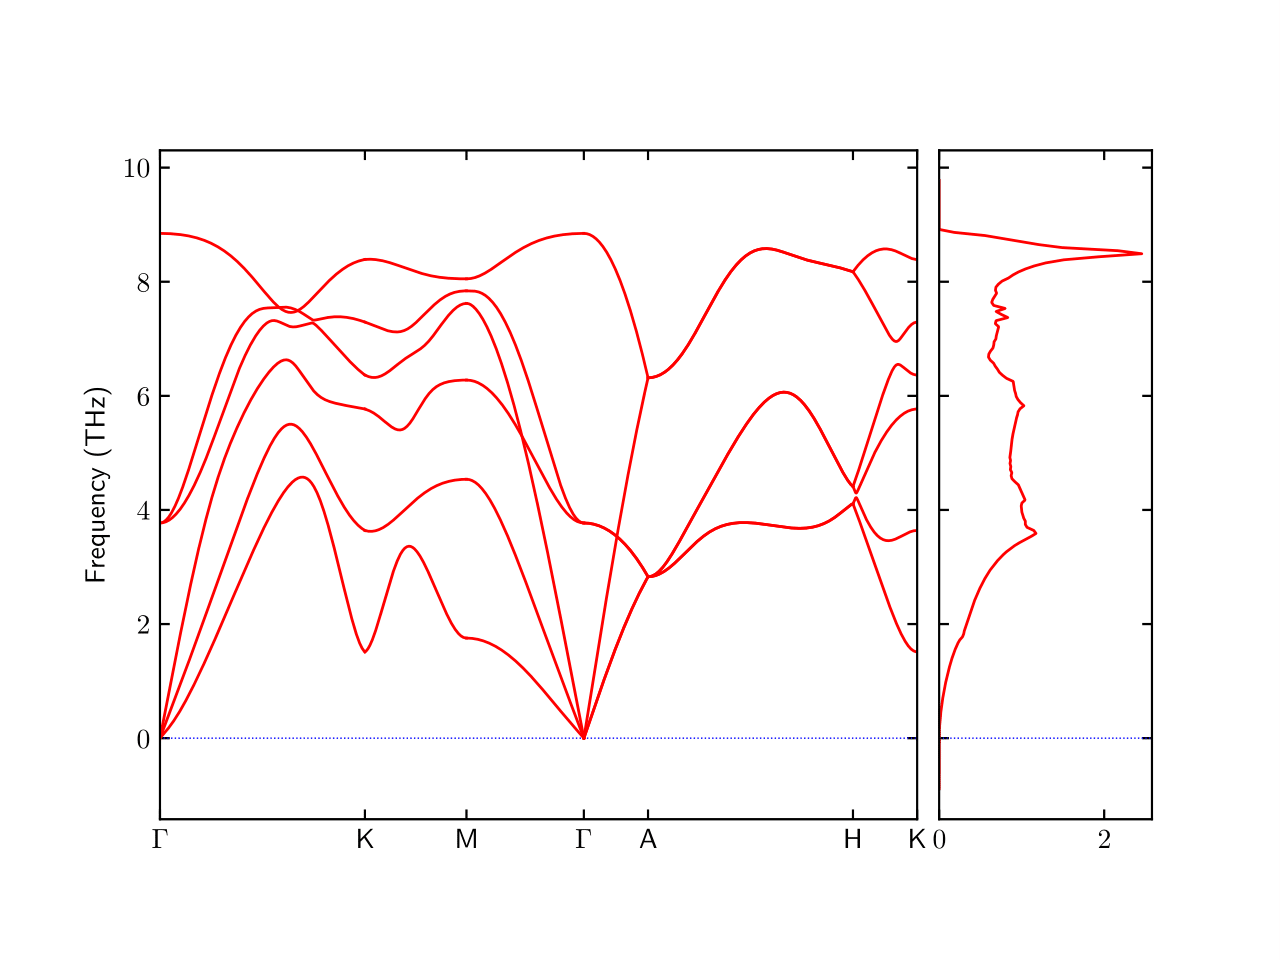
\includegraphics[width=.9\linewidth]{/home/tigany/Documents/docs/Management/Images/hcp-band_dos_2020-04-12.png}
\label{orgf3b8320}
\end{center}

\begin{center}
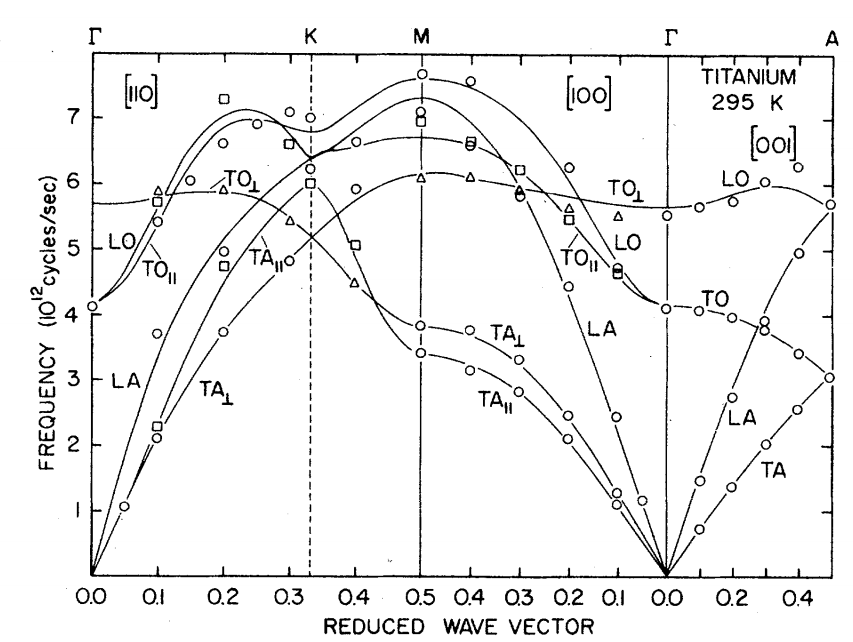
\includegraphics[width=.9\linewidth]{/home/tigany/Documents/docs/Management/Images/experimental_hcp_phonons.png}
\end{center}

\begin{notes}
All frequencies are in THz
\end{notes}

\subsection*{\(\omega\) phase}
\label{sec:org385e39c}
\begin{center}
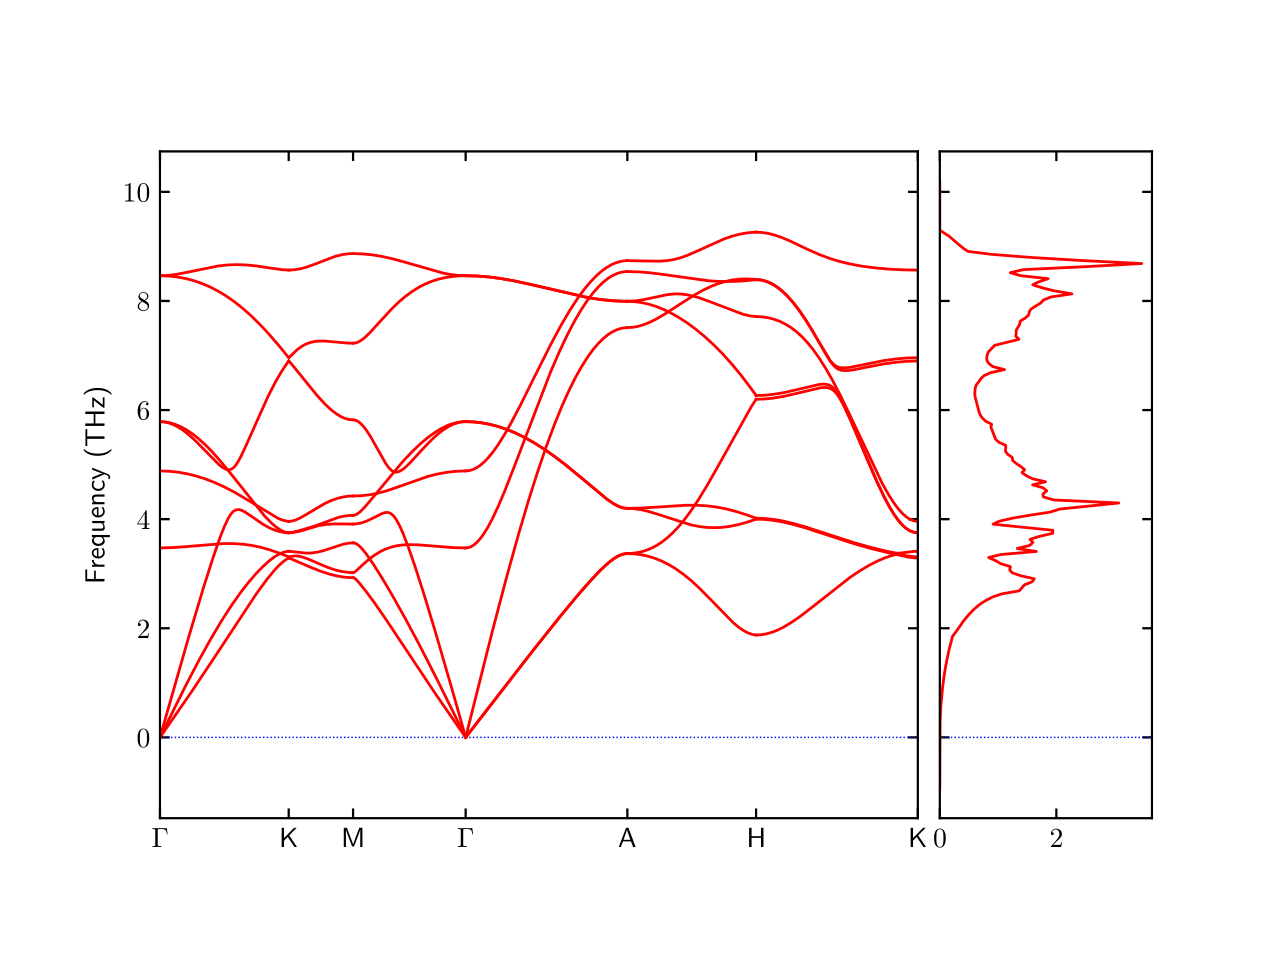
\includegraphics[width=.9\linewidth]{/home/tigany/Documents/docs/Management/Images/omega-band_dos_2020-04-12.png}
\label{orgbd29a9a}
\end{center}

\begin{center}
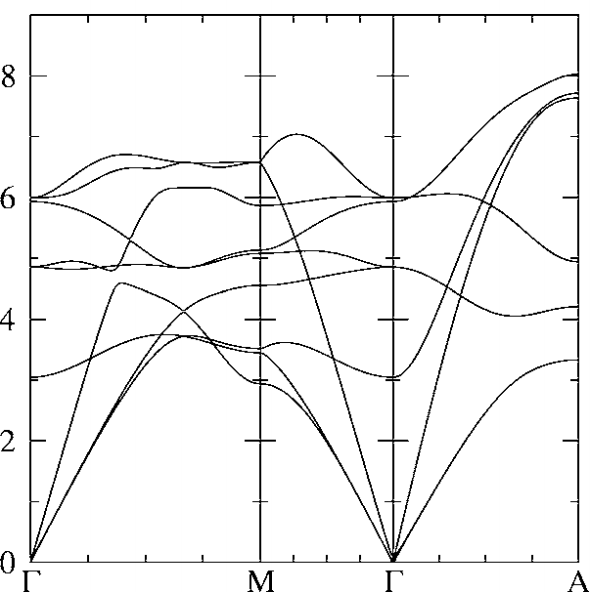
\includegraphics[width=.9\linewidth]{/home/tigany/Documents/docs/Management/Images/omega_phonons_trinkle.png}
\end{center}


\subsection*{\(\beta\) phase}
\label{sec:org149761f}
\begin{center}
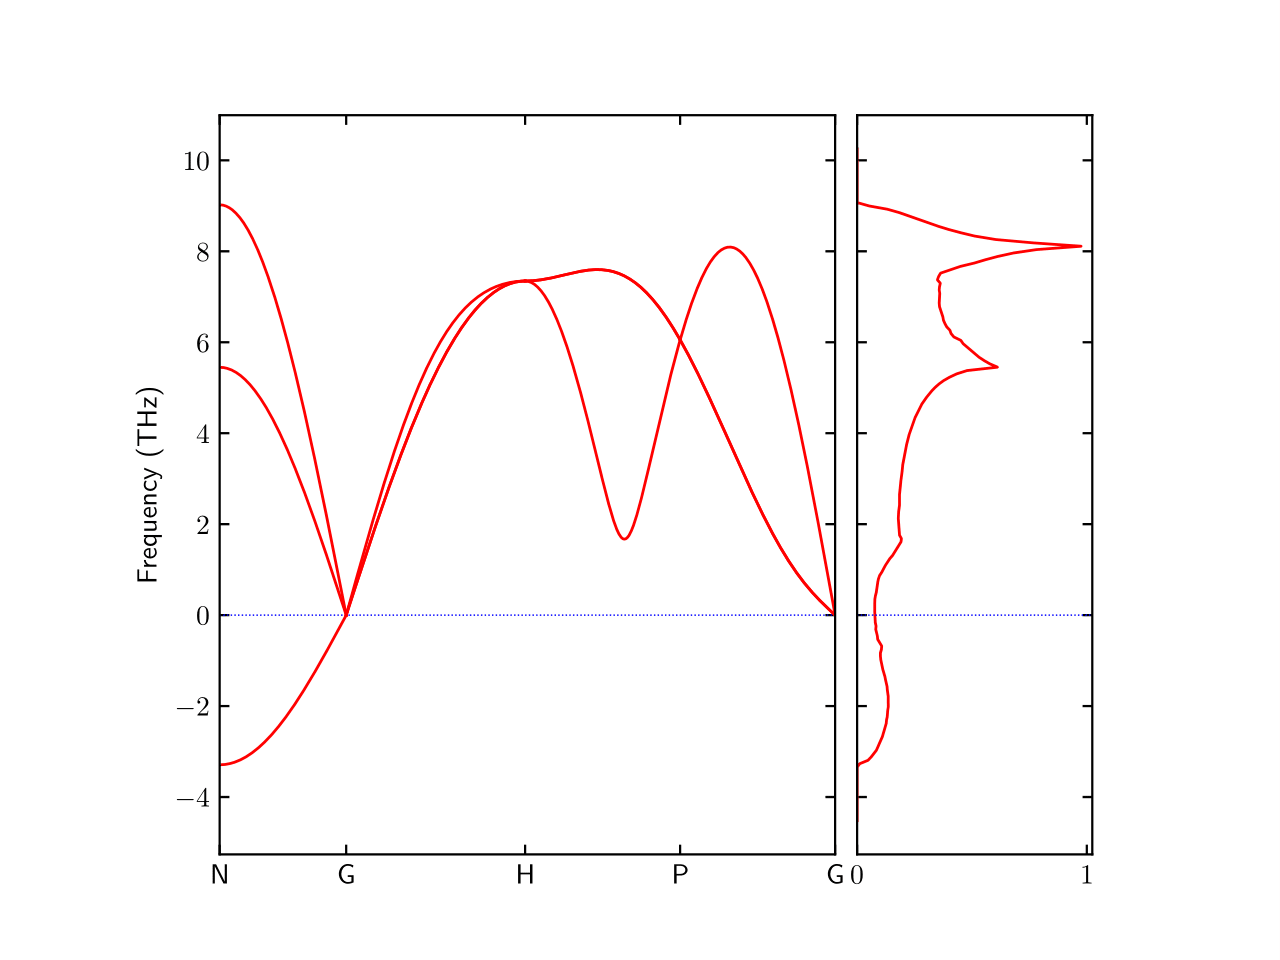
\includegraphics[width=.9\linewidth]{/home/tigany/Documents/docs/Management/Images/bcc-band_dos_2020-04-12.png}
\label{org2e95398}
\end{center}

\begin{center}
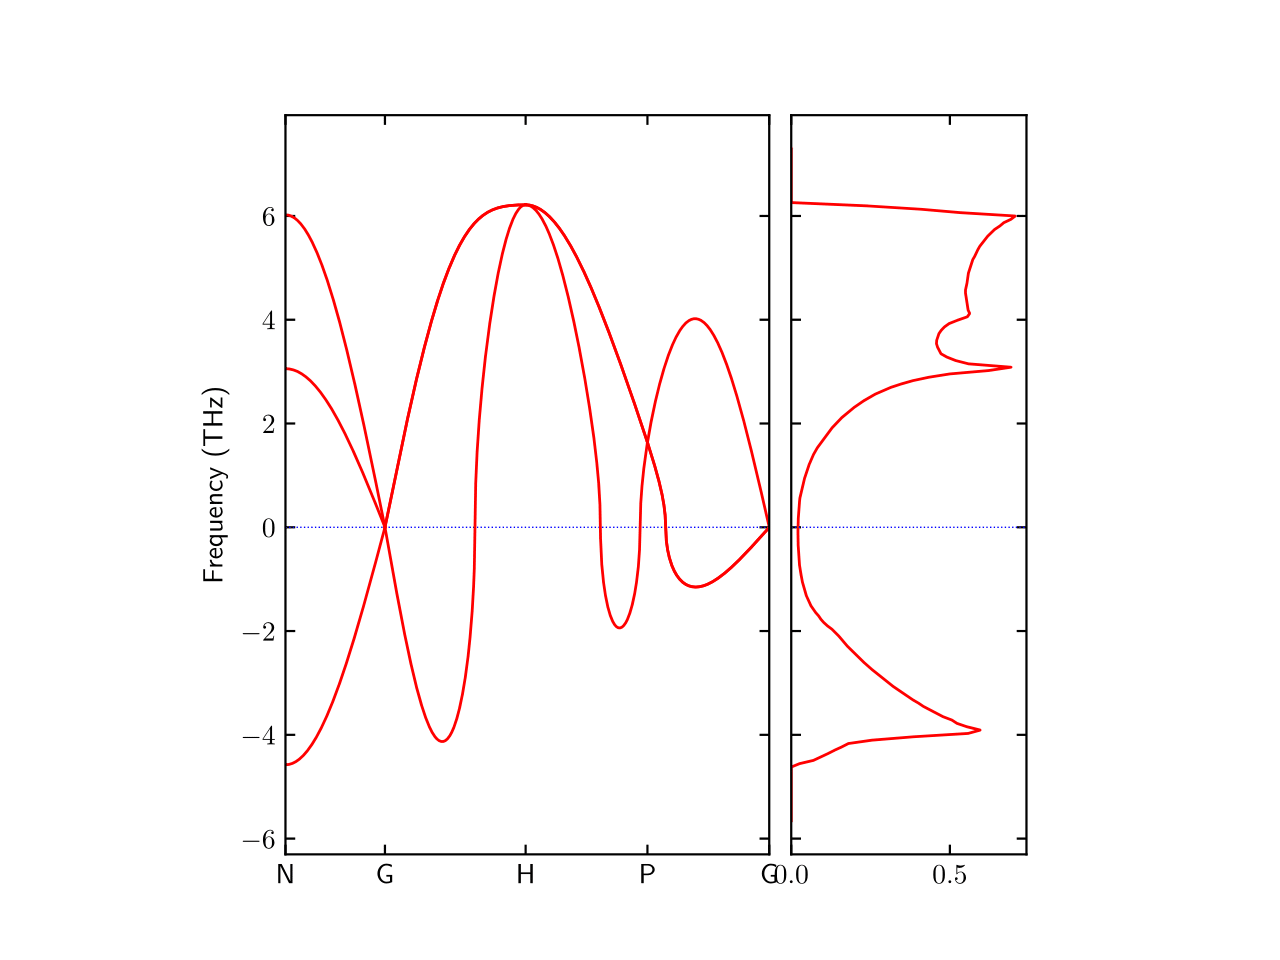
\includegraphics[width=.9\linewidth]{/home/tigany/Documents/docs/Management/Images/bcc-band_dos_dft-1.png}
\end{center}
\section*{Free Energies}
\label{sec:org2dd8063}
\begin{itemize}
\item To find predicted stability of each phase as a function of temperature, one can
use the quasi-harmonic approximation.
\item One finds the volume dependence of the energy, from which we can convert the
Helmholtz free energy into the Gibbs free energy.
\end{itemize}

\subsection*{Gibbs Free Energy}
\label{sec:org2a68e67}
\begin{center}
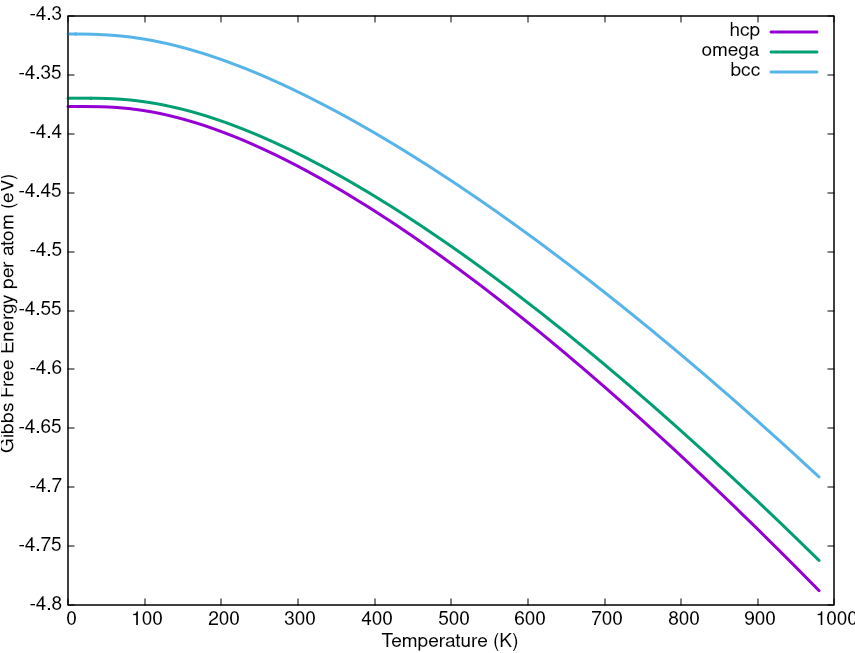
\includegraphics[width=.9\linewidth]{/home/tigany/Documents/docs/Management/Images/gibbs_free_energy_per_atom_2020-04-02.png}
\label{org4758ed3}
\end{center}

\begin{center}
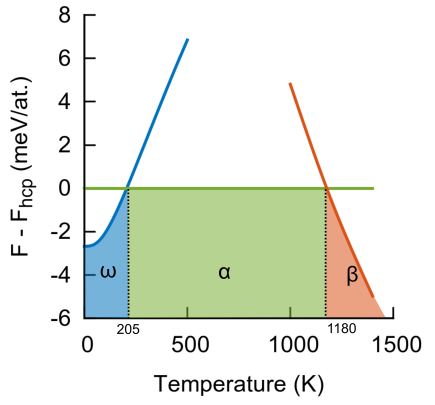
\includegraphics[width=.9\linewidth]{/home/tigany/Documents/docs/Management/Images/matous_free_energy.png}
\end{center}


\subsection*{Thermal Expansion}
\label{sec:org132c9ad}
\begin{center}
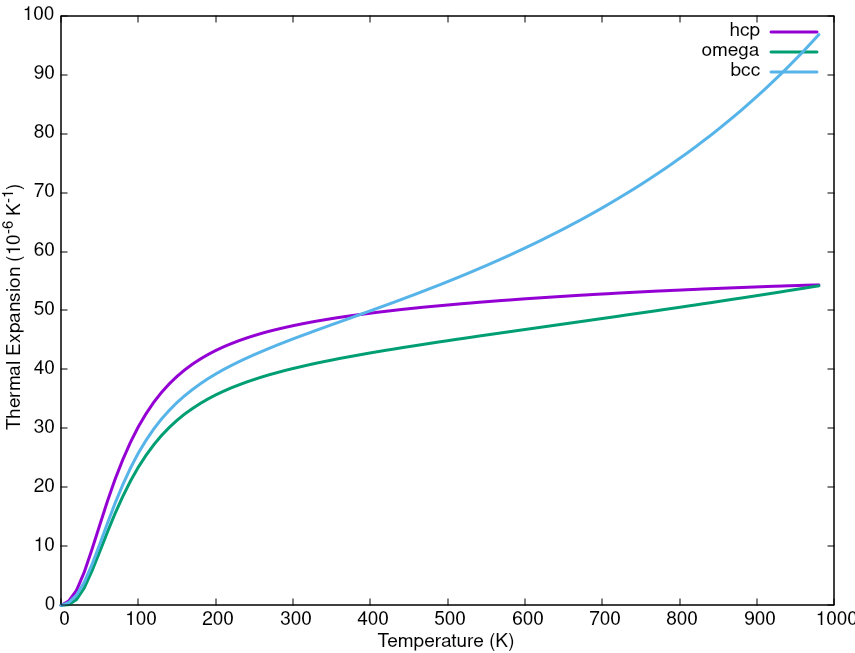
\includegraphics[width=.9\linewidth]{/home/tigany/Documents/docs/Management/Images/thermal_expansion_all_phases_2020-04-02.png}
\label{orgb6e7517}
\end{center}


\begin{center}
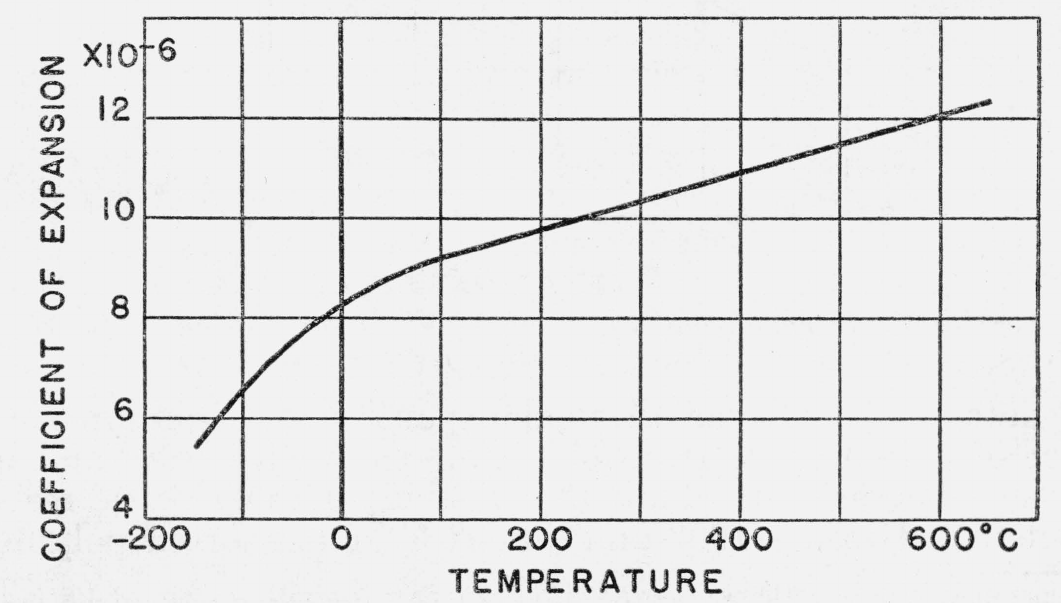
\includegraphics[width=.9\linewidth]{/home/tigany/Documents/docs/Management/Images/thermal_expansion_alpha_ti_exp.png}
\end{center}





\section*{Gamma Surfaces}
\label{sec:org9661bea}


\begin{itemize}
\item \(\gamma\) -surfaces are plots of excess energy with the movement of
atoms on a fault plane.
\item Stable stacking faults correspond to local minima.
\item This provides insight into possible dislocation dissociations.
\end{itemize}

\subsection*{Basal gamma surfaces}
\label{sec:orgcc7662e}


\begin{center}
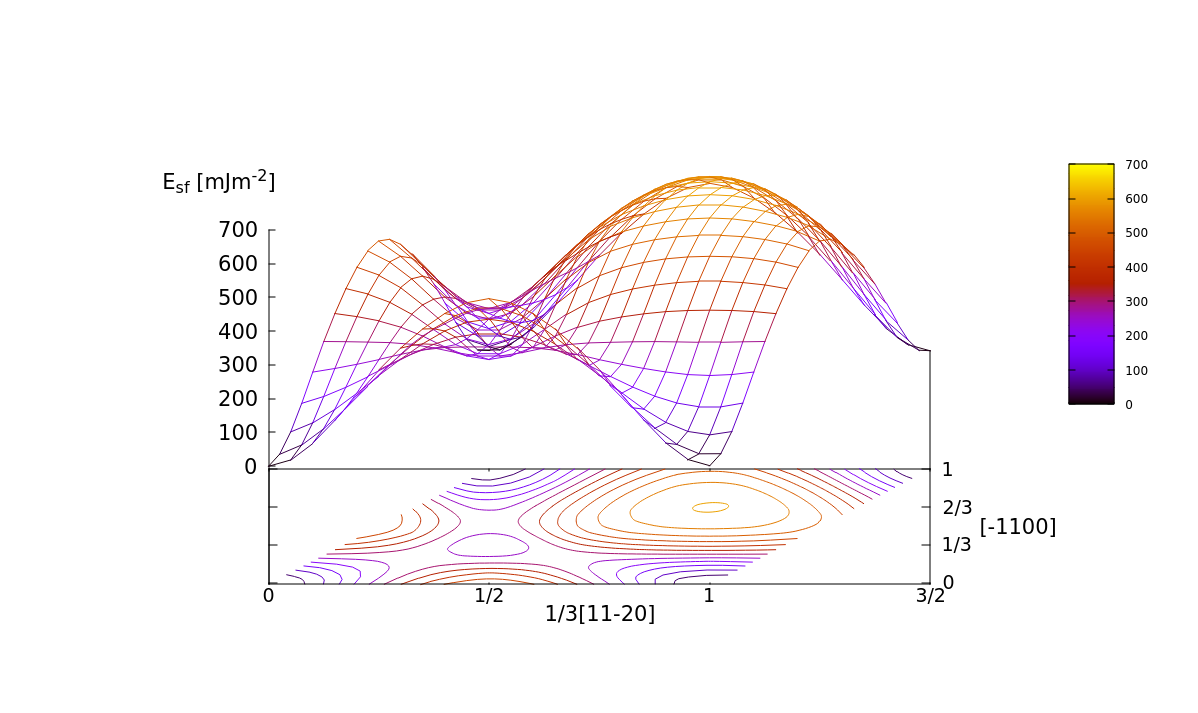
\includegraphics[width=.9\linewidth]{/home/tigany/Documents/docs/Management/Images/basal_gamma_surface_final_model_2020-01-15.png}
\label{org41bb1eb}
\end{center}


\begin{center}
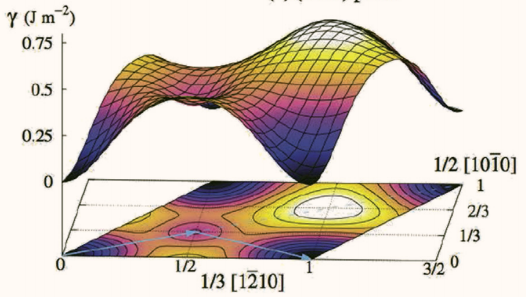
\includegraphics[width=.9\linewidth]{/home/tigany/Documents/docs/Management/Images/rodney_basal_ti_gamma_surface.png}
\end{center}

Expected splitting, (all models): \(\frac{1}{3}[1\bar{2}10] = \frac{1}{3}[1\bar{1}00] +  \frac{1}{3}[0\bar{1}10]\)

\subsection*{Prismatic gamma surfaces}
\label{sec:orgd54b5c5}

\begin{center}
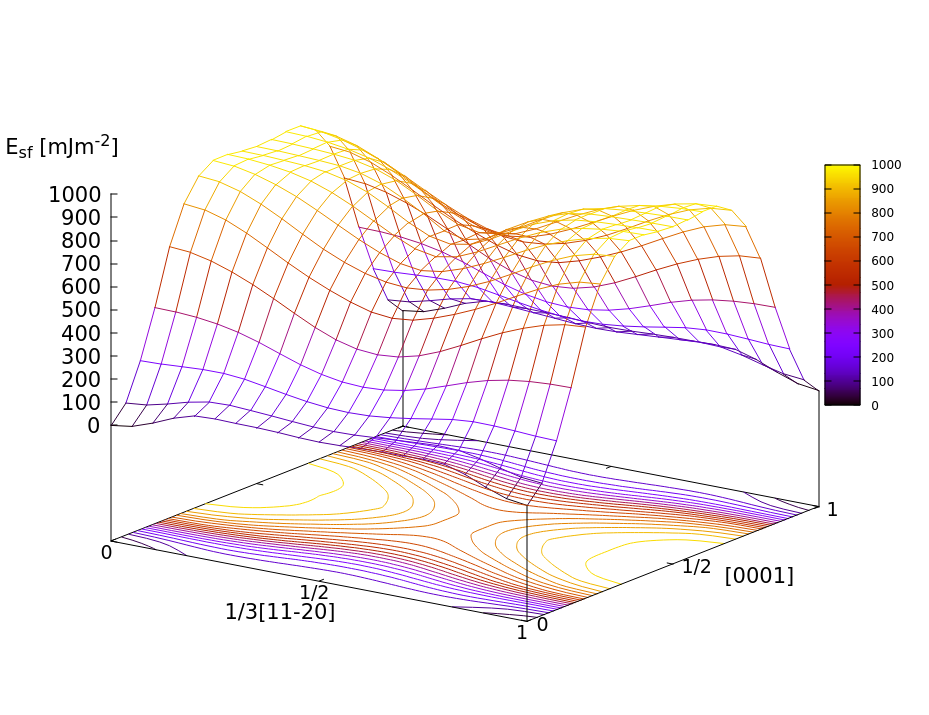
\includegraphics[width=.9\linewidth]{/home/tigany/Documents/docs/Management/Images/prismatic_gamma_surface_final_model_angle_smaller.png}
\end{center}


\begin{center}
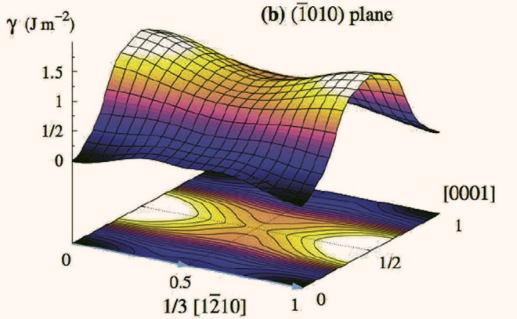
\includegraphics[width=.9\linewidth]{/home/tigany/Documents/docs/Management/Images/rodney_prismatic_ti_gamma_surface.png}
\end{center}


\begin{itemize}
\item Expected splitting (all models): \(\frac{1}{3}[1\bar{2}10] = \frac{1}{6}[1\bar{2}10] + \frac{1}{6}[1\bar{2}10]\)
\end{itemize}

\begin{NOTES}


From TB one can see that the splitting is immediately not exactly the same as
that of DFT. 
\end{NOTES}

\subsection*{Pyramidal gamma surfaces}
\label{sec:org4f6e69f}
\begin{center}
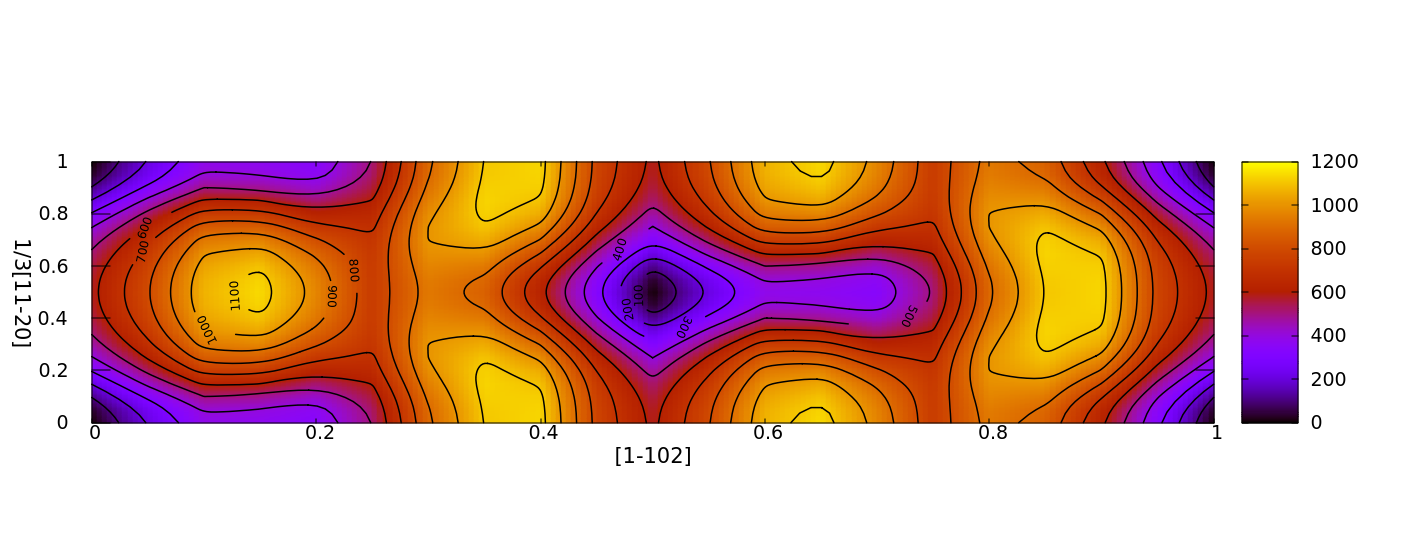
\includegraphics[width=.9\linewidth]{/home/tigany/Documents/docs/Management/Images/rotated_pyramidal_with_contour_wider.png}
\label{org657187c}
\end{center}


\begin{notes}


One can see a saddle point in the interatomic potential and the tb model. So
one can assume that this is a point which relies on subtle electronic
structure methods. Like the prismatic splitting above. 
\end{notes}

\subsection*{Results}
\label{sec:orgd60c7e8}
\begin{center}
\begin{tabular}{lllrll}
 & Plane & Fault & TB & [DFT] & [TB]\\
\hline
 & Basal & \(I_{2}\) & 212 & 260 \(^{[1]}\) & 290 \(^{[2]}\), 110 \(^{[3]}\)\\
\hline
 & Prismatic & \(\gamma_{P}\) & 98 & 250\(^{[1]}\) 233\(^{[4]}\) & 110\(^{[5]}\) ,  260\(^{[3]}\)\\
\hline
 & Pyramidal & \(I_{1}\) & 332 & 288 \(^{[6]}\) & --\\
 &  & \(I_{2}\) & 737 & 788 \(^{[6]}\) & --\\
\end{tabular}
\end{center}


\begin{itemize}
\item Units are in \(mJm^{-2}\). Square brackets denote method from literature.
\item \(^{[1]}\) Benoit (2012), \(^{[2]}\) Bere (1999), \(^{[3]}\) Girshick (1998)
\item \(^{[4]}\) Ackland (1992), \(^{[5]}\) Legrand (1984), \(^{[6]}\) Ready (2019), \(^{[7]}\) Chaari (2014)
\end{itemize}




\section*{Core structures}
\label{sec:orgd30dacd}
\begin{itemize}
\item Dislocation cores are sensitive to boundary conditions.
\item Sufficient resolution of core structure is necessary ascertain how
dislocation glide is modified.
\end{itemize}



\subsection*{\(\frac{1}{3}\langle11\bar{2}0\rangle\) screw}
\label{sec:org4516c51}
\begin{center}
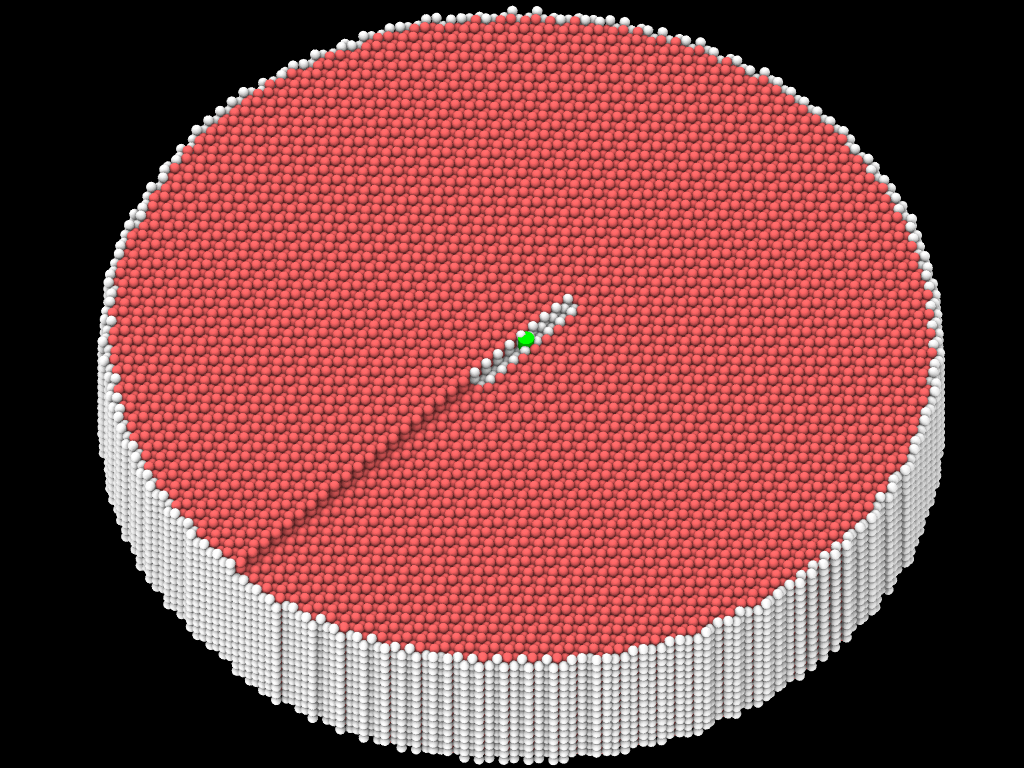
\includegraphics[width=.9\linewidth]{/home/tigany/Documents/docs/Management/Images/bop_dislocation_relaxation_prismatic_partials_larger.png}
\end{center}

\begin{center}
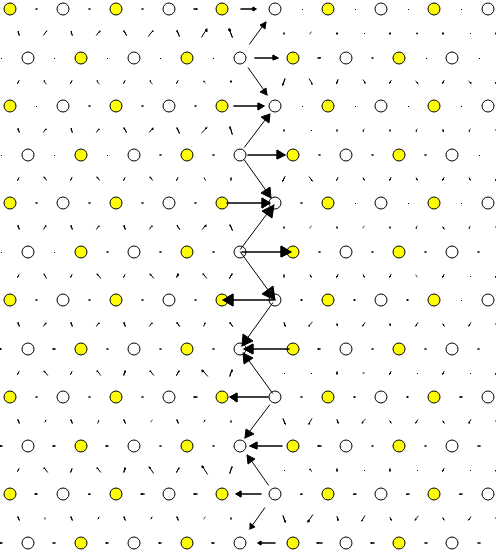
\includegraphics[width=.9\linewidth]{/home/tigany/Documents/docs/Management/Images/ddp_ip5_core_quad.png}
\end{center}

\begin{center}
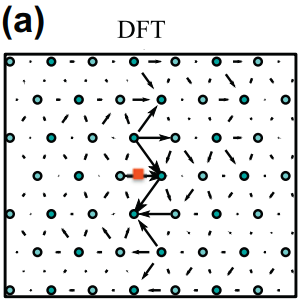
\includegraphics[width=.9\linewidth]{/home/tigany/Documents/docs/Management/Images/ghazisaiedi_trinkle_3_core_just_dft.png}
\end{center}

\begin{center}
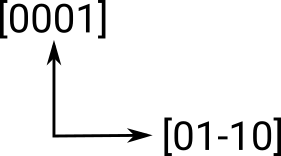
\includegraphics[width=.9\linewidth]{/home/tigany/Documents/docs/Management/Images/coordinate_prismatic_plane.png}
\end{center}


\subsection*{Dislocation Dissociation}
\label{sec:org7a1f3a0}

\begin{itemize}
\item Correct dissociation found of \(\frac{1}{3}[1\bar{2}10] =
     \frac{1}{6}[1\bar{2}10] + \frac{1}{6}[1\bar{2}10]\).
\item Dissociation distance between cores is \(\sim4c\), which is larger
than what is found in DFT.
\end{itemize}


\begin{center}
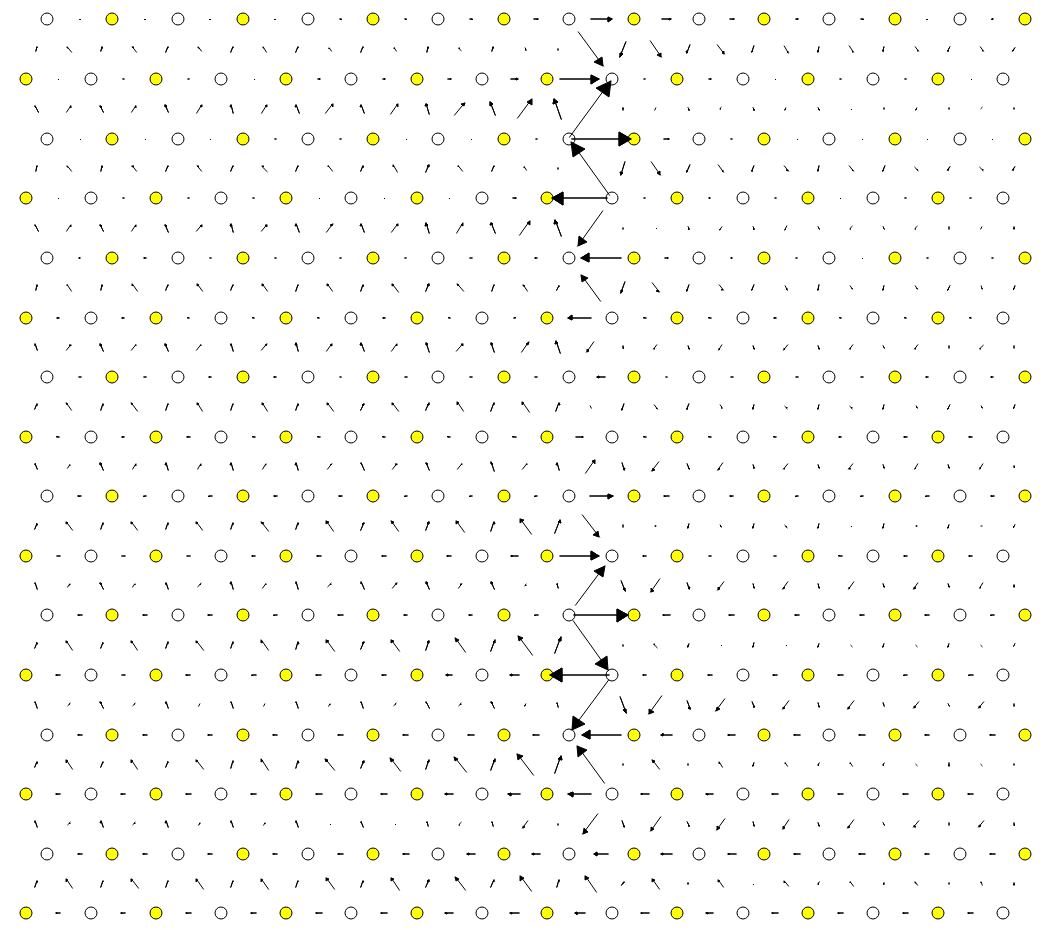
\includegraphics[width=.9\linewidth]{/home/tigany/Documents/docs/Management/Images/final_model_IP1_partial_dd_final.png}
\end{center}



\section*{Peierls Stress}
\label{sec:orgc590617}

\begin{itemize}
\item To find the peierls stress, the critical stress to move a
dislocation upon a glide plane, one can incrementally strain and
relax the simulation cell until the dislocation has been seen to
move to the next peierls valley.
\end{itemize}

\subsection*{Prismatic Peierls Stress}
\label{sec:org7eb3317}

\begin{itemize}
\item Using an increment in the strain of \(\epsilon_{xz}\) by \(1\times 10^{-4}C_{44}'\), the
dislocation moves by c/2 at \(\sigma_{xz}= 0.0012C_{44}'\), giving a Peierls stress of \(\sigma_{xz} =
     2C_{44}\epsilon_{xz}= 0.0923\) GPa.
\item This is half the strain necessary for the MEAM potential of
Trinkle et al.
\end{itemize}


\section*{O-dislocation binding}
\label{sec:org198c47d}

\begin{itemize}
\item 576 atom quadrupolar cell of 1b depth relaxed.
\item Cell replicated three times, giving depth of 3b.
\item O placed in octahedral sites at various distances from the
dislocation core in the middle layer.
\item Interaction energy defined as 

\[ E^{\text{Int}}_{} = E_{\text{disl-O}} -   E_{\text{disl}} -
    E_{\text{perfect-O}} + E_{\text{perfect}} \]
\end{itemize}

\begin{center}
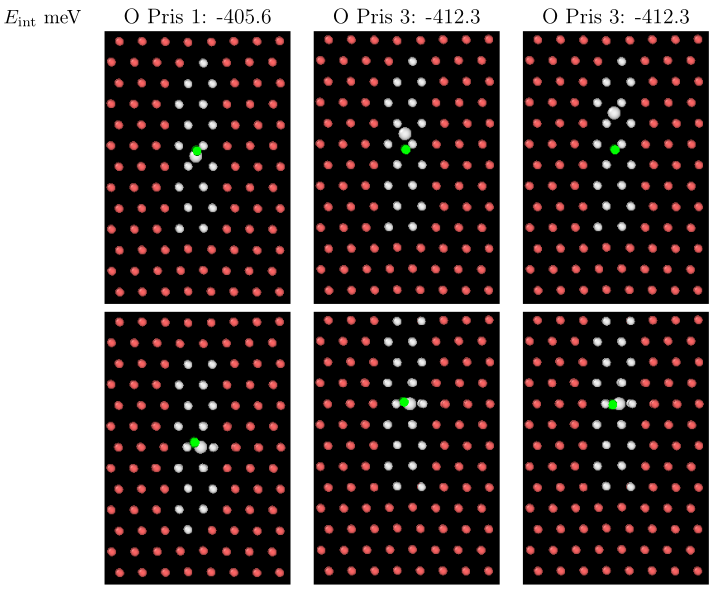
\includegraphics[width=.9\linewidth]{/home/tigany/Documents/docs/Management/Images/prisotioquad.png}
\end{center} v

\begin{center}
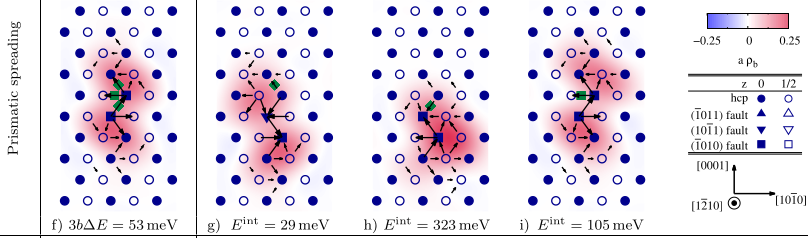
\includegraphics[width=.9\linewidth]{/home/tigany/Documents/docs/Management/Images/chaari_ti-o_dislocation_interactions.png}
\end{center}

\begin{center}
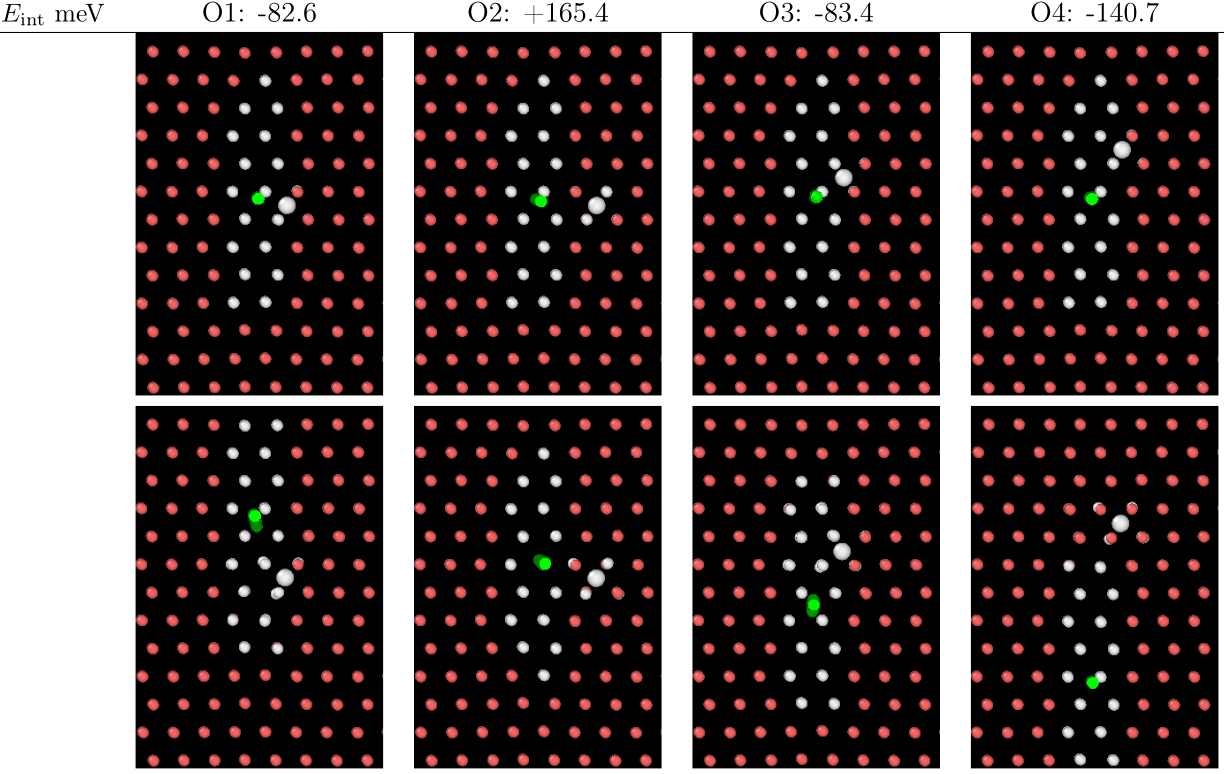
\includegraphics[width=.9\linewidth]{/home/tigany/Documents/docs/Management/Images/ti-o_quadinteractions2.png}
\end{center}

\begin{center}
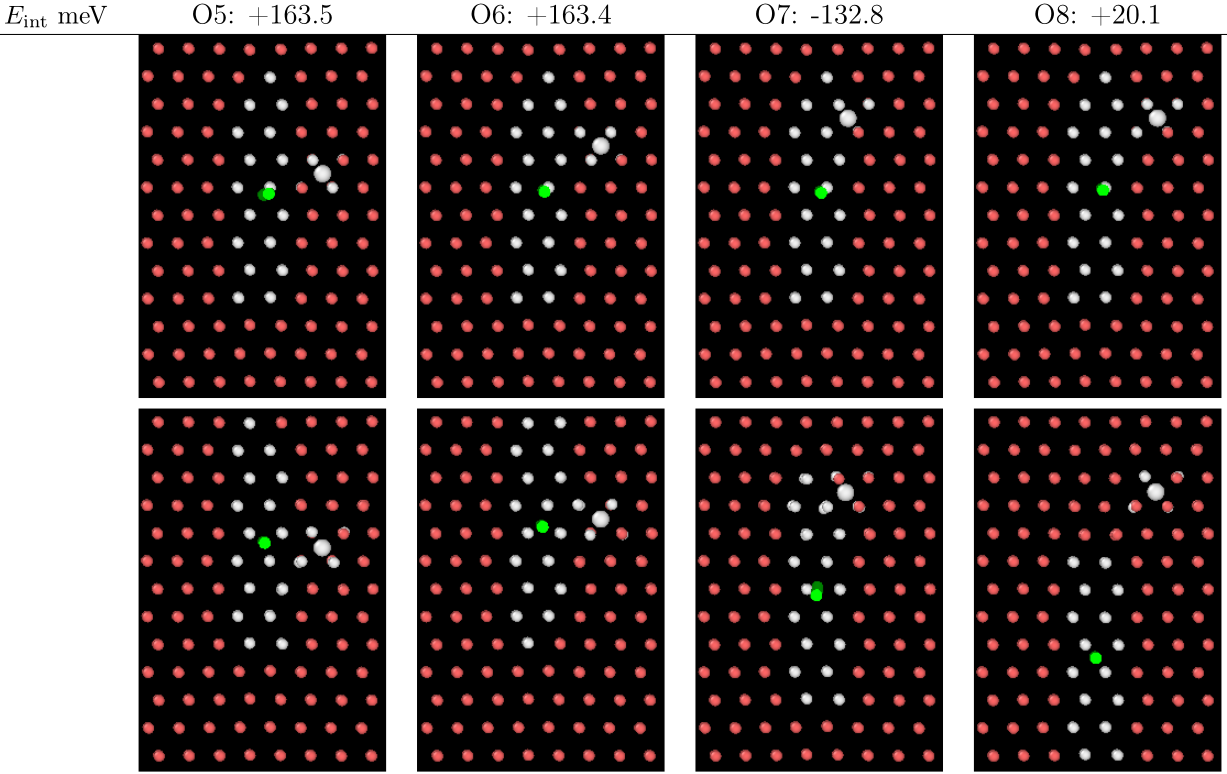
\includegraphics[width=.9\linewidth]{/home/tigany/Documents/docs/Management/Images/ti-o_quadinteractions.png}
\end{center}


\section*{Defects and Defect Clusters}
\label{sec:org1b54115}


\subsection*{Defect Clusters in Ti}
\label{sec:orgba536a8}

\begin{itemize}
\item Increase in oxygen content in Ti-7wt.\%Al causes higher number density of
\(\alpha_2\) precipitates at 550\textdegree{} C (Felicity's results).
\item Oxygen acting as a defactant might stabilise defect complexes (Ti\textsubscript{v} + nO).
\item This can cause more defects resulting in the increased number of precipitates due to more nucleation sites.
\item First starting out with pure Ti and \(\alpha_2\).
\end{itemize}

\subsection*{Vacancy formation Energy}
\label{sec:org96fae6d}

\begin{center}
\begin{tabular}{lr}
\(\Delta E_{\text{f}}^{\text{vacancy}}\) & [eV]\\
\hline
Tight Binding & 2.34\\
GGA-DFT Trinkle (2006) & 2.03\\
GGA-DFT Connetable (2011) & 1.97\\
Exp. Hashimoto (1984) & 1.27\\
\hline
\end{tabular}
\end{center}

\subsubsection*{Dependence on Temperature}
\label{sec:org3347398}
\begin{itemize}
\item Vibrational free energy determined by calculation of dynamical
matrix through atomic displacements by phonopy (\(\sim-0.03\) eV
contribution at \(T=0\)).
\item Configurational entropy given by standard formula. \(S_c^{\text{V}} = k_B
      \text{ln}( N))\)
\end{itemize}

\begin{center}
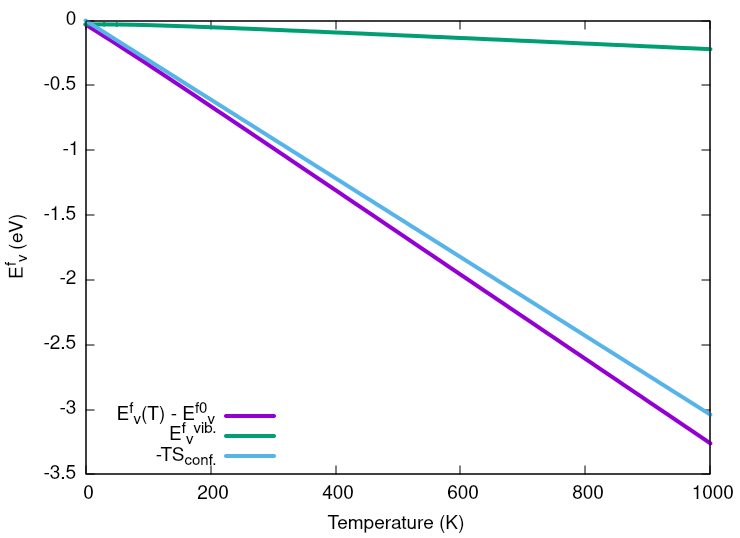
\includegraphics[width=.9\linewidth]{/home/tigany/Documents/docs/Management/Images/vacancy_formation_temperature_dep_contrib_2020-04-13.png}
\end{center}


\subsection*{Oxygen solution Energies}
\label{sec:orgc33659f}
\begin{itemize}
\item Octahedral site for oxygen is most stable, as expected.
\item Tetrahedral is unstable: oxygen prefers a hexahedral site.
\end{itemize}

\begin{center}
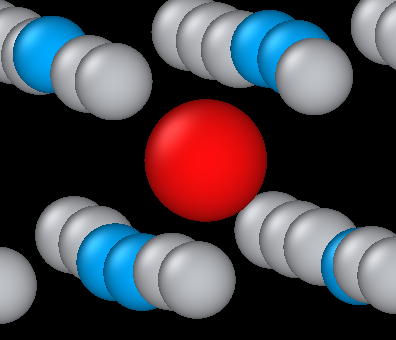
\includegraphics[width=.9\linewidth]{/home/tigany/Documents/docs/Management/Images/final_octahedral_ox_ovito.png}
\end{center}

\begin{center}
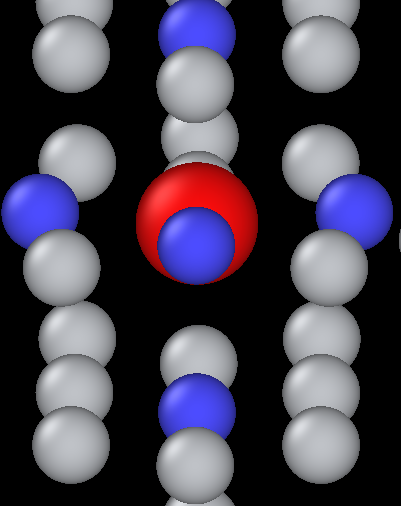
\includegraphics[width=.9\linewidth]{/home/tigany/Documents/docs/Management/Images/final_model_initial_tetra_ox_ovito.png}
\end{center}

\begin{center}
\begin{tabular}{lr}
\(\Delta E_{\text{f}}^{\text{solution}}(\text{Tetra.} - \text{Octa.} )\) & [eV]\\
\hline
Tight Binding & 1.60\\
GGA-DFT Kwasniak (2013) & 1.23\\
\hline
\end{tabular}
\end{center}

\subsubsection*{Other Defects}
\label{sec:orgd310edc}
\begin{itemize}
\item \(\mu_{\text{O}} = 5.6 eV\) from Aksyonov (2016).
\end{itemize}


\begin{center}
\begin{tabular}{ll}
Defect Cluster & Energy (eV)\\
\hline
\(E^{\text{sol}}(H)\) & -  21.783 (DFT: -4.8)\\
\(E^{\text{sol}}(O)\) & -  23.436 (DFT: -5.592)\\
\(E^{\text{sol}}(2O)\) & -  46.806\\
\(E^{\text{sol}}(3O)\) & -  70.437\\
\(E^{\text{sol}}(4O)\) & -  94.070\\
\(E^{\text{sol}}(5O)\) & - 117.581\\
\(E^{\text{sol}}(6O)\) & - 141.148\\
\end{tabular}
\end{center}

\begin{center}
\begin{tabular}{ll}
Defect Cluster & Energy (eV)\\
\hline
\(E^{\text{sol}}(H+V)\) & -  18.905\\
\(E^{\text{sol}}(O+V)\) & -  18.905\\
\(E^{\text{sol}}(2O+V)\) & -  41.910\\
\(E^{\text{sol}}(3O+V)\) & -  66.013\\
\(E^{\text{sol}}(4O+V)\) & -  88.998\\
\(E^{\text{sol}}(5O+V)\) & - 113.649\\
\(E^{\text{sol}}(6O+V)\) & - 137.110\\
\end{tabular}
\end{center}




\subsubsection*{Temperature Dependence}
\label{sec:org921fe98}

\begin{itemize}
\item Introducing \(n_{\text{O}}\) oxygen interstitials into hcp lattice, the
partial configurational entropy is \[ S_{C}^{n_\text{O}} =
      k_{\text{B}}N\text{ln}\Big\{ \frac{\theta(1-\theta)}{(1-2\theta)^2} \Big\}, \]
\item \(\theta = n_{\text{O}}/N\)
\end{itemize}
\begin{center}
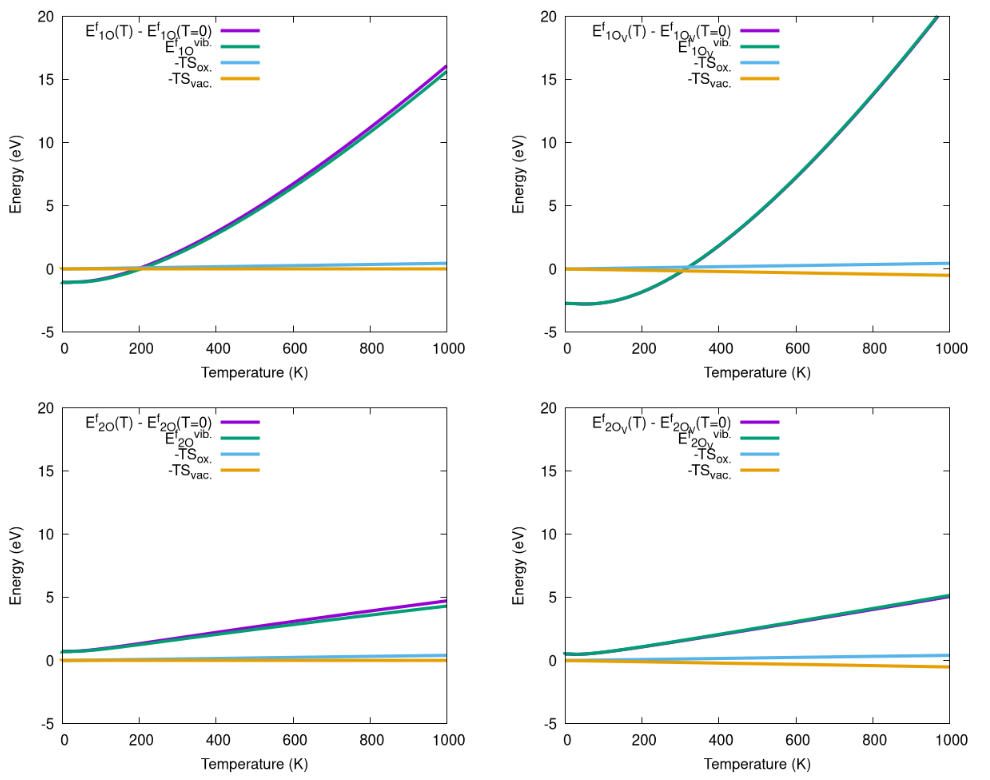
\includegraphics[width=.9\linewidth]{/home/tigany/Documents/docs/Management/Images/defect_clusters_O12V_contribution.png}
\end{center}


\subsubsection*{Vacancy-solute binding energies}
\label{sec:org58773b7}

\begin{itemize}
\item Binding energy here has convention of positive values being
attractive.
\item Here we see that all complexes are unfavourable.
\end{itemize}
\begin{center}
\begin{tabular}{ll}
Defect Cluster & \(E^{\text{bind}}\)\\
\hline
\(E^{\text{b}}(H+V)\) & - 0.530\\
\(E^{\text{b}}(O+V)\) & - 2.183\\
\(E^{\text{b}}(2O+V)\) & - 2.547\\
\(E^{\text{b}}(3O+V)\) & - 2.076\\
\(E^{\text{b}}(4O+V)\) & - 2.724\\
\(E^{\text{b}}(5O+V)\) & - 1.583\\
\(E^{\text{b}}(6O+V)\) & - 1.690\\
\end{tabular}
\end{center}










\subsection*{Molecular Dynamics}
\label{sec:org4c730a7}


\subsection*{Tight-Binding: Future Work}
\label{sec:org92759d0}
\begin{itemize}
\item Finish embedding calculations to see how core structure changes
with O content.
\item Calculate the Peierls barrier on prism, and \(\pi\) planes.
\item Calculate secondary Peierls barrier for kink migration with and without
oxygen.
\item Add rutile layer. See how dislocations and oxygen interact with structure.
\item Simulate high pressure \(\text{Ti-H}_{2}\text{O}\) system.
\end{itemize}


\section*{Defect Clusters}
\label{sec:org47b3c9c}

\begin{itemize}
\item Increase in oxygen content in Ti-7wt.\%Al causes higher number density of
\(\alpha_2\) precipitates at 550\textdegree{} C (Felicity's results).
\item Oxygen acting as a defactant might stabilise defect complexes (Ti\textsubscript{v} + nO).
\item This can cause more defects resulting in the increased number of precipitates due to more nucleation sites.
\item First starting out with pure Ti and \(\alpha_2\). Still working on extension to Ti-7wt.\%Al.
\end{itemize}


\subsection*{Calculation Details}
\label{sec:orgcb9cfe0}
\begin{itemize}
\item Först \emph{et al.} \([6]\) calculated energetics of defect complexes with associated local
force-constant matrix.
\item Partial thermodynamic equilibrium imposed (thermal equilibrium for one species and not the other).
\item Defect concentration plotted as a function of carbon/vacancy concentration
only at 160\textdegree{} C.
\item Extension: apply the quasiharmonic approximation/do thermodynamic integration
for better accuracy at higher temperatures (550\textdegree{} C - 950\textdegree{} C).
\end{itemize}

\([6]\) \emph{Point Defect Concentrations in Metastable Fe-C Alloys}, Först \emph{et
al}, Phys. Rev. Lett. 96, 2006



\subsection*{Plots in Fe-C}
\label{sec:org1247700}
\begin{center}
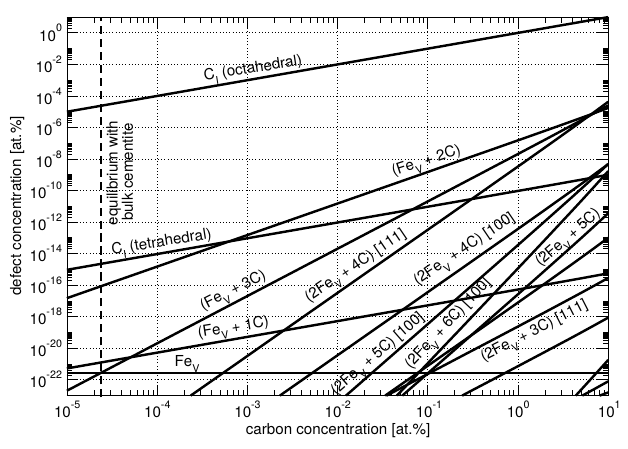
\includegraphics[width=.9\linewidth]{/home/tigany/Documents/docs/Management/Images/forst_defect_concentration_cementite.png}
\label{orgdab65fb}
\end{center}

\begin{center}
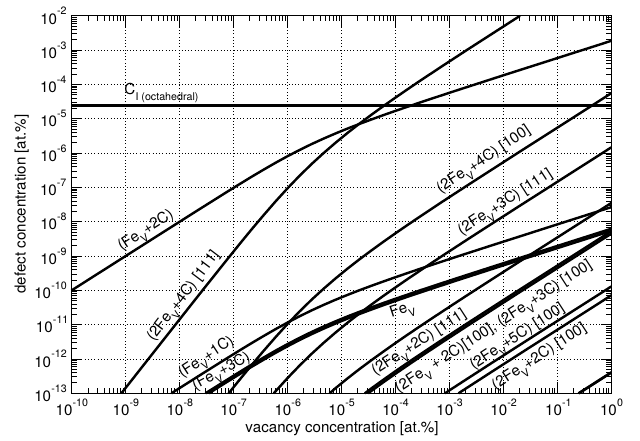
\includegraphics[width=.9\linewidth]{/home/tigany/Documents/docs/Management/Images/forst_defect_concentration_vacancies.png}
\label{org6c22436}
\end{center}


\section*{Future Work}
\label{sec:orgae6cd09}

\begin{itemize}
\item Find peierls barrier for prismatic and pyramidal planes.
\item Elucidate changes in core structure from oxygen near core.
\item Determine at what distance from the core the O-disl. binding energy matches elastic calculations.
\item Find concentration of defect clusters under variation of oxygen and
vacancy concentration.
\end{itemize}

\subsection*{\(\text{Ti}_{3}\text{Al}\)  Cells}
\label{sec:org57103e7}
\begin{center}
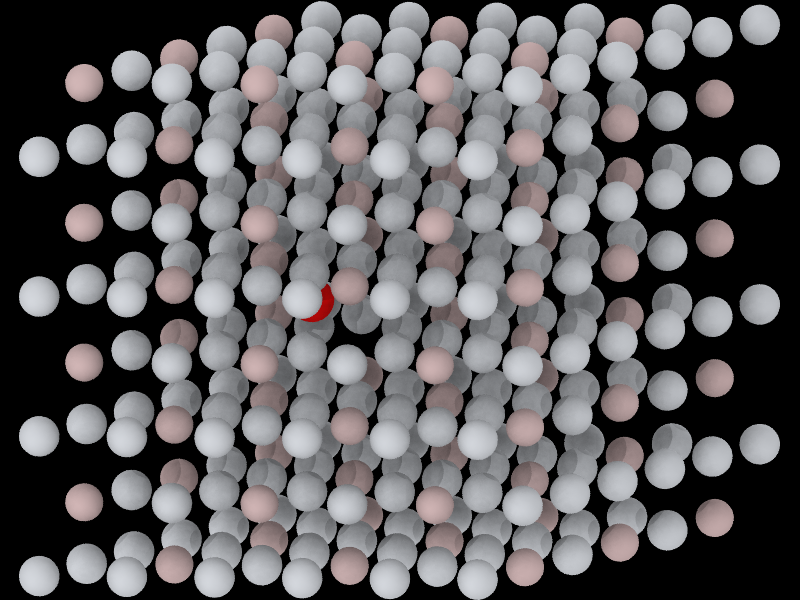
\includegraphics[width=.9\linewidth]{/home/tigany/Documents/docs/Management/Images/ti3al_val_o.png}
\label{orgbbeebc9}
\end{center}

\subsection*{Ti Cells}
\label{sec:org7e75343}


\subsection*{Defect Clusters: Future Work}
\label{sec:orge81b24d}
\begin{itemize}
\item Finish Ti and \(\text{Ti}_{3}\text{Al}\) defect cluster calculations in DFT.
\item Possibly extend to Ti-7wt\%Al with SQS structures.
\item See how much of an effect anharmonicity has on predictions.
\end{itemize}


\section*{Additional references}
\label{sec:org06a518d}

\begin{itemize}
\item Ghazisaeidi, Trinkle (2012), \emph{Core structure of a screw dislocation in Ti from density functional theory and classical potentials}.
\item Rodney, Ventelon (2016), \emph{Ab initio modelling of dislocation core properties
in metals and semiconductors}.
\item Chaari, Clouet (2014), \emph{First order pyramidal slip of 1/3 screw dislocations in zirconium}
\end{itemize}
\end{document}
